\begin{enumerate}[label=\arabic*.,ref=\theenumi]

\numberwithin{equation}{enumi}
\numberwithin{figure}{enumi}

\item For a feedback transconductance amplifier in Fig \ref{fig:fig1}, derive an approximate expression for the closed loop transconductance T for the case of GH $\gg$1. Hence select a value of $R_2$ to obtain T=100 mA/V. If Q is biased to obtain $g_m$ = 1mA/V, specify  the value of the gian $\mu$ of the differential amplifier to obtain an amount of feedback of 60 dB. If Q has $r_o$ = 50 k$\ohm$ find the $R_{out}$.
\begin{figure}[!ht]
	\begin{center}
		\resizebox{\columnwidth}{!}{\ctikzset{tripoles/mos style/arrows}
\usetikzlibrary{decorations.markings}
\begin{circuitikz}
\ctikzset{bipoles/length=1cm}

\draw 
(0,0) node[op amp,yscale=-1.0] (opamp) {\rotatebox{180}{\reflectbox{$\mu$}}}
(1.5,0) node[nmos,](Q){}
(opamp.+) (-0.85, +0.35) -- (-3, +0.35) to [V=$V_s$] (-3,-1) to (-3,-1) node[ground]{}
(opamp.-) (-0.85, -0.35) -- (-0.85, -1.7) to [R=$R_3$] (-0.85,-4) to (-0.85,-4) node[ground]{}
(opamp.-) (-0.85, -0.35) -- (-0.85, -1.7) to [R=$R_2$] (1.5,-1.7) to (1.5,-1.7) 
(1.5,-0.5) to (1.5, -1.7) to [R=$R_1$] (1.5,-4) node[ground]{}

node at(-1.2,-1.7){$V_f$}
node at(1.8,-0.6){$I_o$}
node at (-0.2,-3.3){$100\ohm$}
node at (2.2,-3.3){$100\ohm$}
 ;



\draw[thick,->,>=stealth] (1.5,-0.9) -- (1.5,-1);

\draw[thick,->,>=stealth] (Q.D);


\end{circuitikz}
}
	\end{center}
\caption{Complete Circuit}
\label{fig:fig1}
\end{figure}



\solution


\begin{figure}[!ht]
	\begin{center}
		\resizebox{\columnwidth}{!}{\begin{circuitikz}
\ctikzset{bipoles/length=1cm}

\draw 
(0,0)  to[R=$R_2$] (3,0) to[R=$R_1$] (3,-2) node[ground]{}
(0,0) to [R=$R_3$](0,-2)  (0,-2) node[ground]{}
(3,0) -- (4,0){}
(4,-2) node[ground]{}
(4,-2) to[I=$I_o$] (4,0){}

node at(0,0.3){$V_f$}
node at(3,0.3){$V_x$}


;\end{circuitikz}}
	\end{center}
\caption{Feedback Circuit}
\label{fig:fig2}
\end{figure}



\begin{align}
H = \frac{V_f}{I_o}
\label{eq: eq1}
\end{align}

From Fig.\ref{fig:fig2}
\begin{align}
    V_x = ((R_2 + R_3) \| R_1) I_o 
    \label{eq: eq2}
\end{align} 

\begin{align}
V_f = I_f R_3
\label{eq: eq3}
\end{align} 
\begin{align}
V_x - V_f = R_2 I_f
\label{eq: eq4}
\end{align} 

From equations \ref{eq: eq1} to \ref{eq: eq4} we get

\begin{align}
    H = \frac{V_f}{I_o}=\frac{R_1 R_3}{R_1+R_2+R_3}
    \label{eq:eq5}
\end{align}

As GH $\gg$ 1 ,

\begin{align}
    T = \frac{1}{H}
    \label{eq:eq6}
\end{align}

For T = 100 mA/V,

\begin{align}
    R_2 = 800 \ohm
    \label{eq:eq7}
\end{align}
$\implies H=10$


\begin{figure}[!ht]
	\begin{center}
		\resizebox{\columnwidth}{!}{\begin{circuitikz}
\ctikzset{bipoles/length=1cm}
\draw
(0,0) to[short,*-*] (1,0){}
(0.5,0) -- (0.5,-0.5) to[R, l_=$R_{id}$] (0.5,-1.5) (0.5,-1.5)--(0.5,-3.5) 
(0.5,-3.5) to [R=$R_3$] (0.5,-4.5){}
(0.5,-4.5) node[ground]{}

(0.5,-3) -- (2.5,-3) to [R=$R_{2}$] (3.5,-3) -- (5.5,-3) 

(2,0) to[R=$r_{01}$,*-*] (4,0){}
(2,0) to[cV=$\mu V_i$] (2,-2)  {}
(2,-2) node[ground]{}
(5.5,0) to[I=$g_{m}V_{gs}$] (5.5,-2){}
(5.5,0)--((5.5,1) --(6,1) node[ground]{}
(5.5,0) -- (7,0) to[R=$r_{0}$] (7,-2) -- (5.5,-2){}
(5.5,-2) to[short, i = $I_{o}$] (5.5,-3.5) to[R=$R_1$] (5.5,-4.5) node[ground]{}


node at(4.1,-1) {$V_{gs}$}

node at(4.1,-0.2) {$+$}
node at(4.1,-2) {$-$}
node at(0,0.25) {$V_s$}

node at(0.7,-0.3) {$+$}
node at(0.7,-1.7) {$-$}
node at(0.9,-1.2) {$V_i$}

;\end{circuitikz}}
	\end{center}
\caption{Small signal model}
\label{fig:fig3}
\end{figure}


\begin{align}
    G = \frac{I_o}{V_i} 
    \label{eq;eq8}
\end{align}

From Fig. \ref{fig:fig3} we can see that
 
\begin{align}
    V_{gs} = \mu V_i - V_x
    \label{eq;eq9}
\end{align}

\begin{align}
    g_mV_{gs} - \frac{V_x}{r_o} = I_o
    \label{eq;eq10}
\end{align}

From equations \ref{eq;eq9} to \ref{eq;eq10}
\begin{align}
    G = \frac{I_o}{V_i} = \frac{g_m \mu r_o}{r_o + (1+g_m r_o)((R_2+R_3)\|R_1) }
    \label{eq:eq11}
\end{align}

Given GH = 60dB,
\begin{align}
    20\log_{10} GH = 60 dB
    \label{eq:eq12}
\end{align}

\begin{align}
\implies G=100
\end{align}

Substituting the values in the Eq. \ref{eq:eq11}
\begin{align}
    \mu = 109180
\end{align}
For output reistance,
\begin{align}
    R_o = r_o + g_m r_o((R_2+R_3)\|R_1) + ((R_2+R_3)\|R_1)    
    \label{eq:eq13}
\end{align}
Substituting the values in Eq.\ref{eq:eq13} 
\begin{align}
    R_o=54.59k\ohm
\end{align}
\begin{align}
R_{out} = R_o(1+GH)    
\end{align}

$\implies$  $R_{out}$ = 54.64 M$\ohm$


\begin{table}[!ht]
\centering
%%%%%%%%%%%%%%%%%%%%%%%%%%%%%%%%%%%%%%%%%%%%%%%%%%%%%%%%%%%%%%%%%%%%%%
%%                                                                  %%
%%  This is the header of a LaTeX2e file exported from Gnumeric.    %%
%%                                                                  %%
%%  This file can be compiled as it stands or included in another   %%
%%  LaTeX document. The table is based on the longtable package so  %%
%%  the longtable options (headers, footers...) can be set in the   %%
%%  preamble section below (see PRAMBLE).                           %%
%%                                                                  %%
%%  To include the file in another, the following two lines must be %%
%%  in the including file:                                          %%
%%        \def\inputGnumericTable{}                                 %%
%%  at the beginning of the file and:                               %%
%%        \input{name-of-this-file.tex}                             %%
%%  where the table is to be placed. Note also that the including   %%
%%  file must use the following packages for the table to be        %%
%%  rendered correctly:                                             %%
%%    \usepackage[latin1]{inputenc}                                 %%
%%    \usepackage{color}                                            %%
%%    \usepackage{array}                                            %%
%%    \usepackage{longtable}                                        %%
%%    \usepackage{calc}                                             %%
%%    \usepackage{multirow}                                         %%
%%    \usepackage{hhline}                                           %%
%%    \usepackage{ifthen}                                           %%
%%  optionally (for landscape tables embedded in another document): %%
%%    \usepackage{lscape}                                           %%
%%                                                                  %%
%%%%%%%%%%%%%%%%%%%%%%%%%%%%%%%%%%%%%%%%%%%%%%%%%%%%%%%%%%%%%%%%%%%%%%



%%  This section checks if we are begin input into another file or  %%
%%  the file will be compiled alone. First use a macro taken from   %%
%%  the TeXbook ex 7.7 (suggestion of Han-Wen Nienhuys).            %%
\def\ifundefined#1{\expandafter\ifx\csname#1\endcsname\relax}


%%  Check for the \def token for inputed files. If it is not        %%
%%  defined, the file will be processed as a standalone and the     %%
%%  preamble will be used.                                          %%
\ifundefined{inputGnumericTable}

%%  We must be able to close or not the document at the end.        %%
	\def\gnumericTableEnd{\end{document}}


%%%%%%%%%%%%%%%%%%%%%%%%%%%%%%%%%%%%%%%%%%%%%%%%%%%%%%%%%%%%%%%%%%%%%%
%%                                                                  %%
%%  This is the PREAMBLE. Change these values to get the right      %%
%%  paper size and other niceties.                                  %%
%%                                                                  %%
%%%%%%%%%%%%%%%%%%%%%%%%%%%%%%%%%%%%%%%%%%%%%%%%%%%%%%%%%%%%%%%%%%%%%%

	\documentclass[12pt%
			  %,landscape%
                    ]{report}
       \usepackage[latin1]{inputenc}
       \usepackage{fullpage}
       \usepackage{color}
       \usepackage{array}
       \usepackage{longtable}
       \usepackage{calc}
       \usepackage{multirow}
       \usepackage{hhline}
       \usepackage{ifthen}

	\begin{document}


%%  End of the preamble for the standalone. The next section is for %%
%%  documents which are included into other LaTeX2e files.          %%
\else

%%  We are not a stand alone document. For a regular table, we will %%
%%  have no preamble and only define the closing to mean nothing.   %%
    \def\gnumericTableEnd{}

%%  If we want landscape mode in an embedded document, comment out  %%
%%  the line above and uncomment the two below. The table will      %%
%%  begin on a new page and run in landscape mode.                  %%
%       \def\gnumericTableEnd{\end{landscape}}
%       \begin{landscape}


%%  End of the else clause for this file being \input.              %%
\fi

%%%%%%%%%%%%%%%%%%%%%%%%%%%%%%%%%%%%%%%%%%%%%%%%%%%%%%%%%%%%%%%%%%%%%%
%%                                                                  %%
%%  The rest is the gnumeric table, except for the closing          %%
%%  statement. Changes below will alter the table's appearance.     %%
%%                                                                  %%
%%%%%%%%%%%%%%%%%%%%%%%%%%%%%%%%%%%%%%%%%%%%%%%%%%%%%%%%%%%%%%%%%%%%%%

\providecommand{\gnumericmathit}[1]{#1} 
%%  Uncomment the next line if you would like your numbers to be in %%
%%  italics if they are italizised in the gnumeric table.           %%
%\renewcommand{\gnumericmathit}[1]{\mathit{#1}}
\providecommand{\gnumericPB}[1]%
{\let\gnumericTemp=\\#1\let\\=\gnumericTemp\hspace{0pt}}
 \ifundefined{gnumericTableWidthDefined}
        \newlength{\gnumericTableWidth}
        \newlength{\gnumericTableWidthComplete}
        \newlength{\gnumericMultiRowLength}
        \global\def\gnumericTableWidthDefined{}
 \fi
%% The following setting protects this code from babel shorthands.  %%
 \ifthenelse{\isundefined{\languageshorthands}}{}{\languageshorthands{english}}
%%  The default table format retains the relative column widths of  %%
%%  gnumeric. They can easily be changed to c, r or l. In that case %%
%%  you may want to comment out the next line and uncomment the one %%
%%  thereafter                                                      %%
\providecommand\gnumbox{\makebox[0pt]}
%%\providecommand\gnumbox[1][]{\makebox}

%% to adjust positions in multirow situations                       %%
\setlength{\bigstrutjot}{\jot}
\setlength{\extrarowheight}{\doublerulesep}

%%  The \setlongtables command keeps column widths the same across  %%
%%  pages. Simply comment out next line for varying column widths.  %%
\setlongtables

\setlength\gnumericTableWidth{%
	53pt+%
	93pt+%
0pt}
\def\gumericNumCols{2}
\setlength\gnumericTableWidthComplete{\gnumericTableWidth+%
         \tabcolsep*\gumericNumCols*2+\arrayrulewidth*\gumericNumCols}
\ifthenelse{\lengthtest{\gnumericTableWidthComplete > \linewidth}}%
         {\def\gnumericScale{\ratio{\linewidth-%
                        \tabcolsep*\gumericNumCols*2-%
                        \arrayrulewidth*\gumericNumCols}%
{\gnumericTableWidth}}}%
{\def\gnumericScale{1}}

%%%%%%%%%%%%%%%%%%%%%%%%%%%%%%%%%%%%%%%%%%%%%%%%%%%%%%%%%%%%%%%%%%%%%%
%%                                                                  %%
%% The following are the widths of the various columns. We are      %%
%% defining them here because then they are easier to change.       %%
%% Depending on the cell formats we may use them more than once.    %%
%%                                                                  %%
%%%%%%%%%%%%%%%%%%%%%%%%%%%%%%%%%%%%%%%%%%%%%%%%%%%%%%%%%%%%%%%%%%%%%%

\ifthenelse{\isundefined{\gnumericColA}}{\newlength{\gnumericColA}}{}\settowidth{\gnumericColA}{\begin{tabular}{@{}p{53pt*\gnumericScale}@{}}x\end{tabular}}
\ifthenelse{\isundefined{\gnumericColB}}{\newlength{\gnumericColB}}{}\settowidth{\gnumericColB}{\begin{tabular}{@{}p{93pt*\gnumericScale}@{}}x\end{tabular}}

\begin{tabular}[c]{%
	b{\gnumericColA}%
	b{\gnumericColB}%
	}

%%%%%%%%%%%%%%%%%%%%%%%%%%%%%%%%%%%%%%%%%%%%%%%%%%%%%%%%%%%%%%%%%%%%%%
%%  The longtable options. (Caption, headers... see Goosens, p.124) %%
%	\caption{The Table Caption.}             \\	%
% \hline	% Across the top of the table.
%%  The rest of these options are table rows which are placed on    %%
%%  the first, last or every page. Use \multicolumn if you want.    %%

%%  Header for the first page.                                      %%
%	\multicolumn{2}{c}{The First Header} \\ \hline 
%	\multicolumn{1}{c}{colTag}	%Column 1
%	&\multicolumn{1}{c}{colTag}	\\ \hline %Last column
%	\endfirsthead

%%  The running header definition.                                  %%
%	\hline
%	\multicolumn{2}{l}{\ldots\small\slshape continued} \\ \hline
%	\multicolumn{1}{c}{colTag}	%Column 1
%	&\multicolumn{1}{c}{colTag}	\\ \hline %Last column
%	\endhead

%%  The running footer definition.                                  %%
%	\hline
%	\multicolumn{2}{r}{\small\slshape continued\ldots} \\
%	\endfoot

%%  The ending footer definition.                                   %%
%	\multicolumn{2}{c}{That's all folks} \\ \hline 
%	\endlastfoot
%%%%%%%%%%%%%%%%%%%%%%%%%%%%%%%%%%%%%%%%%%%%%%%%%%%%%%%%%%%%%%%%%%%%%%

\hhline{|-|-}
	 \multicolumn{1}{|p{\gnumericColA}|}%
	{\gnumericPB{\centering}\gnumbox{\textbf{Parameter}}}
	&\multicolumn{1}{p{\gnumericColB}|}%
	{\gnumericPB{\centering}\gnumbox{\textbf{Value}}}
\\


\hhline{|--|}
	 \multicolumn{1}{|p{\gnumericColA}|}%
	{\gnumericPB{\raggedright}\gnumbox[l]{$1/g_{m}$}}
	&\multicolumn{1}{p{\gnumericColB}|}%
	{\gnumericPB{\raggedright}\gnumbox[l]{$1k\Omega$}}
\\
\hhline{|--|}
	 \multicolumn{1}{|p{\gnumericColA}|}%
	{\gnumericPB{\raggedright}\gnumbox[l]{$G$}}
	&\multicolumn{1}{p{\gnumericColB}|}%
	{\gnumericPB{\raggedright}\gnumbox[l]{$100A/V$}}
\\
\hhline{|--|}
	 \multicolumn{1}{|p{\gnumericColA}|}%
	{\gnumericPB{\raggedright}\gnumbox[l]{$H$}}
	&\multicolumn{1}{p{\gnumericColB}|}%
	{\gnumericPB{\raggedright}\gnumbox[l]{$10V/A$}}
\\
\hhline{|--|}
	 \multicolumn{1}{|p{\gnumericColA}|}%
	{\gnumericPB{\raggedright}\gnumbox[l]{$GH$}}
	&\multicolumn{1}{p{\gnumericColB}|}%
	{\gnumericPB{\raggedright}\gnumbox[l]{$1000$}}
\\
\hhline{|--|}
	 \multicolumn{1}{|p{\gnumericColA}|}%
	{\gnumericPB{\raggedright}\gnumbox[l]{$T$}}
	&\multicolumn{1}{p{\gnumericColB}|}%
	{\gnumericPB{\raggedright}\gnumbox[l]{$0.1A/V$}}

\\
\hhline{|--|}
	 \multicolumn{1}{|p{\gnumericColA}|}%
	{\gnumericPB{\raggedright}\gnumbox[l]{$R_{o}$}}
	&\multicolumn{1}{p{\gnumericColB}|}%
	{\gnumericPB{\raggedright}\gnumbox[l]{$54.59k\Omega$}}
\\
\hhline{|--|}
	 \multicolumn{1}{|p{\gnumericColA}|}%
	{\gnumericPB{\raggedright}\gnumbox[l]{$R_{out}$}}
	&\multicolumn{1}{p{\gnumericColB}|}%
	{\gnumericPB{\raggedright}\gnumbox[l]{$54.64M\Omega$}}
\\
\hhline{|-|-|}
\end{tabular}

\ifthenelse{\isundefined{\languageshorthands}}{}{\languageshorthands{\languagename}}
\gnumericTableEnd
\caption{}
\label{table: Output_Table}
\end{table}
    
The following code generates the values
\begin{lstlisting}
codes/ee18btech11041.py
\end{lstlisting}

The following code generates results from spice solution

\begin{lstlisting}
codes/spice/ee18btech11041_spice.py
\end{lstlisting}

\begin{figure}[!ht]
\centering
\includegraphics[width=\columnwidth]{./figs/H1.eps}
\caption{}
\label{fig:fig4}
\end{figure}


\begin{figure}[!ht]
\centering
\includegraphics[width=\columnwidth]{./figs/G1.eps}
\caption{}
\label{fig:fig5}
\end{figure}


\begin{figure}[!ht]
\centering
\includegraphics[width=\columnwidth]{./figs/T1.eps}
\caption{}
\label{fig:fig4}
\end{figure}


\end{enumerate}
